%%%%%%%%%%%%%%%%%%%%%%%%%%%%%%%%%%%%%%%%%%%%%%%%
% chapter1.tex                                 %
% Contains formatting and content of chapter 1 %
%%%%%%%%%%%%%%%%%%%%%%%%%%%%%%%%%%%%%%%%%%%%%%%%
\chapter{Introduction and Motivation}
\newpage

\section{Introduction}
In Super Smash Bros. Melee (or colloquially known as just ``Melee'') for the Nintendo GameCube, there are 26 characters to choose from, including fan-favorites like Mario and Luigi, to less known characters like Ness and Ice Climbers. In competitive Melee, each player has four lives, also known as stocks. A player wins by depleting all of their opponents stocks before losing theirs.

\indent Typically, in competitive games or sports, each individual or team has equal access to the same moves and techniques. For example, in chess, each player has the same number and types of pieces. In game theory, this is an example of a symmetric game, in which the players have the same strategy set \citep{GameTheoryInAction}. However, in fighting games, each character has a unique moveset that gives them strengths and weaknesses. This is an example of an asymmetric game, in which each character has a unique strategy and set of options that can be employed. Certain characters have swords or projectiles, allowing them to attack opponents from a distance. Some characters are fast, but easy to knock off the stage, while others are slow, but more resilient to being defeated.

\indent Additionally, Melee is unique from other fighting games, in that it is what is known as a platform fighting game. Typically, fighting games are played on a two-dimensional plane with no frills. The goal is to deplete the health of your opponent. In Melee, the goal is to knock your opponent off of the stage to deplete their stocks. Each stage has unique properties that can affect how certain characters play. Characteristics such as platforms, stage transformations, and other interactable elements affect how players approach matchups and can directly affect gameplay. It is agreed upon in the community that certain stages are better for certain characters due to the tools available to the character.

\indent Because of the asymmetric nature of Melee's characters, it is natural to assume that some characters perform better against others due to having a superior toolkit in a given matchup. To express how strong a character is, players will create a ``matchup chart'' or ``matchup spread'' for the character. This is a measurement of a character's probability of winning against other characters in the roster. When designing a matchup chart, it is typically assumed that the players of each character are of equal skill level. Matchup charts are also typically designed based on the perception of how character perform against one another, given their respective toolkits and performance on certain stages. There is typically little to no formal statistical analysis when designing these spreads.

\indent While some matchup charts are expressed using +/- 1, 2,\dots, this is not as descriptive as to how favorable or unfavorable a matchup may be. We can also use explicit probabilities when describing a matchup. Formally, let us define a matchup of character A against character B. When discussing this matchup, we would say ``Charcter A's matchup against Character B is $x/y$,'' where $x$ is the probability that character A would win, $y$ is the probability that character B would win, and $x+y=100$. For example, an even matchup would be designated as ``50/50''. A slightly favorable matchup would be ``55/45'', while a heavily unfavorable matchup may be expressed as ``35/65''.
% Blah blah blah.  Here is an example of how to include and cite a figure: see Figure~\ref{fig:example_figure}
% \begin{figure}[H]
% \center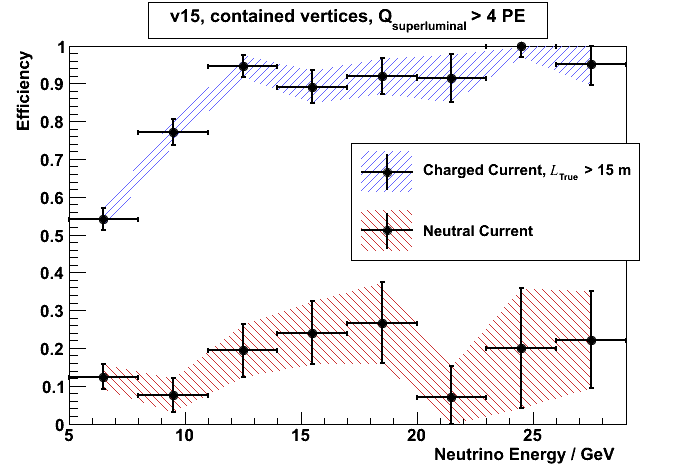
\includegraphics[width=0.4\textwidth]{figures/ExampleFigure.png}
% \caption[Caption to go in list of figures]{Caption to go underneath figure}
% \label{fig:example_figure}
% \end{figure}
\section{Motivation}
A tier list is an ordered list of characters, where each character is ranked based on how strong they are relative to the rest of the cast of characters. Tier lists are often subjective, and they will change over time as the strategies for each character develops over time.

\indent One of the most prominent matchups in competitive melee is Fox vs. Marth. Both of these characters have sat near the top of almost every competitive tier list for over two decades. Both characters have been extremely successful, and many players have piloted the characters to major tournament victories. They each have strong toolkits, and the ability to perform well against any character in the game. However, there has been debate in the Melee community about how Fox and Marth perform against each other.

\indent Most players would argue that the matchup is even. Each charcter has tools in their moveset to exploit the other character's weaknesses. However, top Melee players have expressed different opinions. The most infamous claim was made by the player William ``Leffen'' Hjelte. Leffen, a Fox player, argued that Marth is favored in the matchup 60/40, and it became somewhat of a joke in the Melee community.

\indent I thought that this debate would be interesting to approach from a Bayesian lens. Given expert prior beliefs on the matchup, we could use results from individual matches to determine a more statistically sound matchup spread for a character. Furthermore, Melee has many characters that get less usage due to being considered weaker than most choices. Thus, there is little data for some of these more obscure matchups. Bayesian methods thrive in this environment, allowing us to define such matchup spreads for less-used characters.
% Blah blah blah. Here's an example of a table: see Table~\ref{tab:best_values}.

% \begin{table}[H]
% \centering\onehalfspacing
% \vline
% \begin{tabular}{c c c}
% \hline
% \textbf{Parameter} & \vline & \textbf{Current Best Value}\\
% \hline
% $\Delta m^2_{21}$ & \vline & $7.50^{+0.19}_{-0.20} \times 10^{-3}\;\mathrm{eV}^2$\\
% $|\Delta m^2_{32}|$ & \vline & $2.32^{+0.12}_{-0.08} \times 10^{-5}\;\mathrm{eV}^2$\\
% $\sin^2{(\theta_{12})}$ & \vline & $0.857^{+0.023}_{-0.025}$\\
% $\sin^2{(2\theta_{23})}$ & \vline & $>0.95$\\
% $\sin^2{(\theta_{13})}$ & \vline &  $0.098\pm 0.013$\\
% \hline\end{tabular}\vline
% \captionsetup{width=0.86\textwidth}
% \caption[Name of table for list of tables]{Name of table for caption above table}
% \label{tab:best_values}
% \end{table}

% Here's an example of an equation and some math:
% \begin{equation}
%   U = \begin{pmatrix} c_{12}c_{13} & s_{12}c_{13} & s_{13}e^{i\delta}\\
%     -s_{12}c_{23} - c_{12}s_{23}s_{13}e^{i\delta} & c_{12}c_{23} - s_{12}s_{23}s_{13}e^{i\delta} & s_{23}c_{13}\\
%     s_{12}s_{23} - c_{12}c_{23}s_{13}e^{i\delta} & -c_{12}s_{12} - s_{12}c_{23}s_{13}e^{i\delta} & c_{23}c_{13}
%   \end{pmatrix},
% \end{equation}
% with $c_{ij} = \cos{\theta_{ij}}$ and $s_{ij} = \sin{\theta_{ij}}$.

% Here's an example citation: \citep{PDG}.
